Para a problemática de uma fazenda vertical autônoma orientada por redes neurais foi definida uma metodologia baseada no ciclo Planejar-Fazer-Verificar-Agir (do inglês, Plan-Do-Check-Act ou PDCA) e consiste em a) revisão bibliográfica; b) planejamento da solução lógica do sistema; c) definição das tecnologias, layout do sistema e funcionalidades e d) prototipação.
\begin{figure}[H]
    \centering
    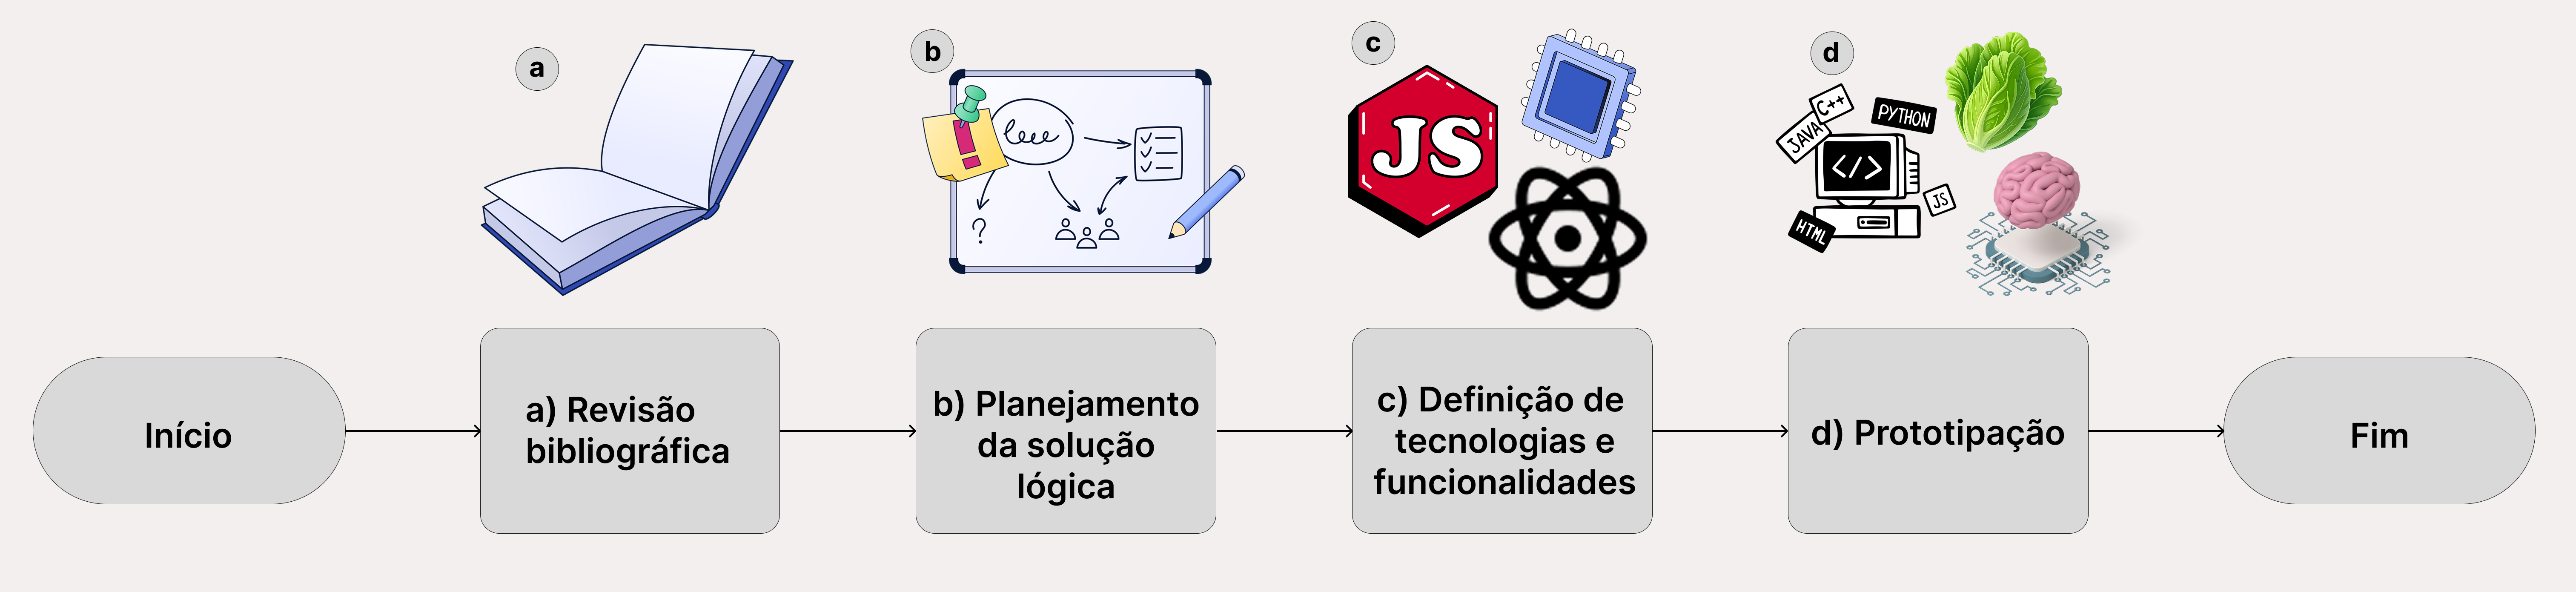
\includegraphics[scale=0.08]{Illustrations/Figura 1.png} % sem extensão se for .png
    \caption{Metodologia adotada para o desenvolvimento do sistema de fazenda vertical autônoma com redes neurais, organizada em quatro etapas sequenciais.
}
    \label{fcht:figura1}
    % \SourceOrNote{Autoria Própria (2024)} % só se esse comando estiver definido
\end{figure}

Após a etapa a) verificação da literatura existente (Estado da Arte), a etapa b) planejamento indicou duas possibilidades: na Figura 2 a fazenda vertical (1) envia, por meio de sensores IoT de nível de água, os dados atuais de fluxo de água e fertilização para um banco de dados na nuvem (2). Estes dados podem ser acessados pelo cliente, por meio de software, onde o usuário pode diretamente tomar a decisão de como devem operar o fluxo de água e fertilização da fazenda, recomeçando o ciclo.


\begin{figure}[H]
    \centering
    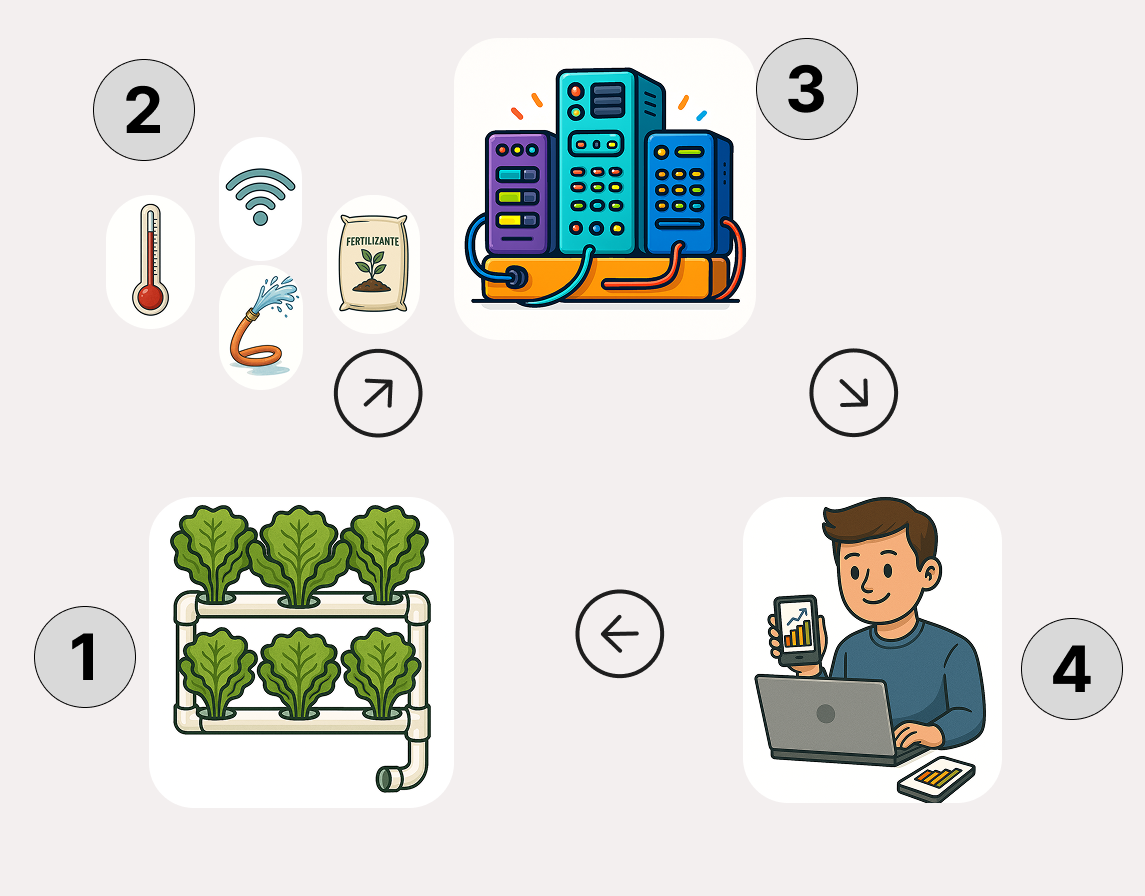
\includegraphics[scale=0.2]{Illustrations/Figura 2.png} % sem extensão se for .png
    \caption{Exemplo de funcionamento do sistema proposto utilizando 4 etapas, mantendo a tomada de decisão sob controle do usuário.}
    \label{fcht:figura2}
    % \SourceOrNote{Autoria Própria (2024)} % só se esse comando estiver definido
\end{figure}


Também é possível que a fazenda vertical (1) envie os dados de fertilizantes e fluxo de água (2) para um banco de dados na nuvem (3). Porém quem faz a avaliação e tomada de decisão com base nos dados é uma Rede Neural (4), recomeçando o ciclo. Assim o cliente apenas participa do ciclo caso queira (conforme Figura 3).

\begin{figure}[H]
    \centering
    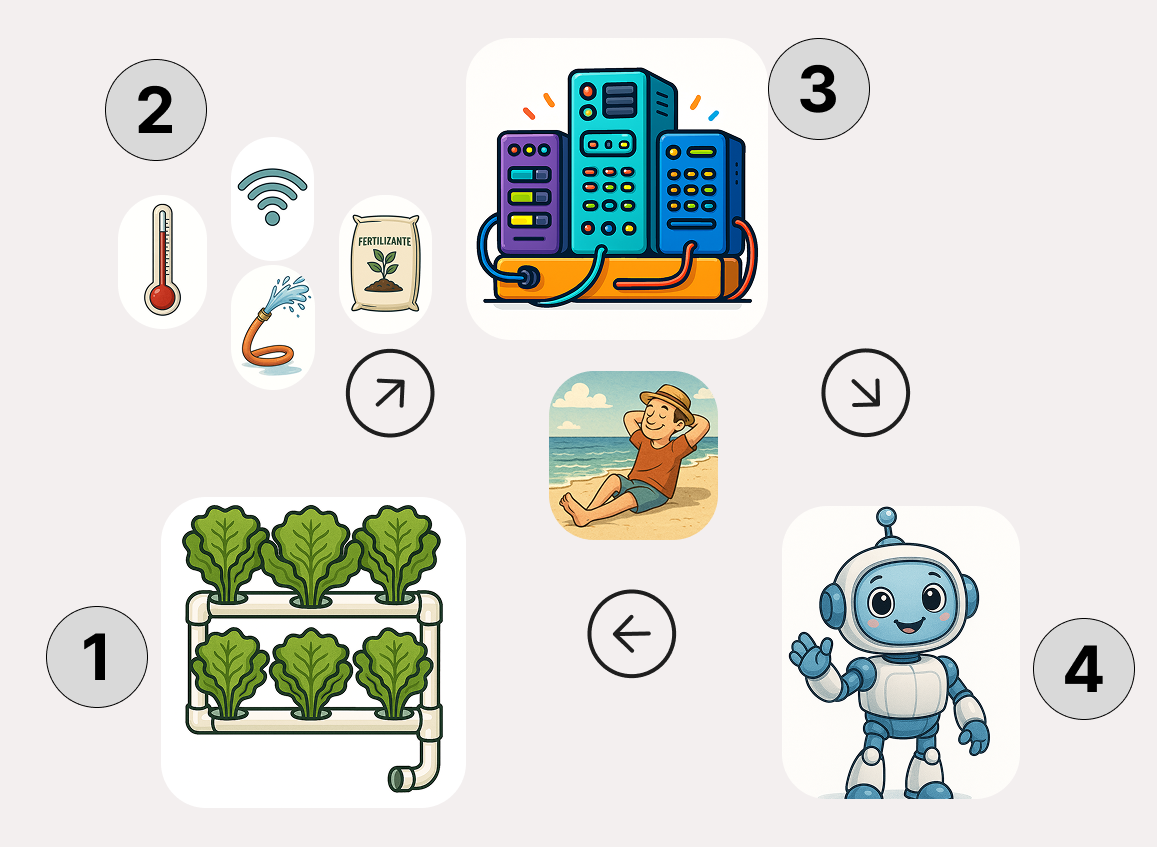
\includegraphics[scale=0.2]{Illustrations/Figura 3.png} % sem extensão se for .png
    \caption{Exemplo de funcionamento do sistema proposto}
    \label{fcht:figura3}
    % \SourceOrNote{Autoria Própria (2024)} % só se esse comando estiver definido
\end{figure}

Na etapa c) Definição das tecnologias, layout do sistema e funcionalidades, primeiramente foi escolhido o Figma (uma plataforma online e gratuita) para desenvolvimento do design e validação dos fluxos. Para o desenvolvimento da API (do inglês, Application Programming Interface, Interface de Programação de Aplicativos), responsável pela integração entre os sistemas e usuário, foi escolhido o Javascript (graças a compatibilidade com diversos dispositivos e vasto acervo de bibliotecas e frameworks) utilizando Node.js (ambiente de execução JavaScript de prototipagem rápida, integração natural com bancos de dados, demanda de poucos recursos de hardware e escalável), React (biblioteca JavaScript usada para criar interfaces de usuário baseada em atualizações rápidas, componentes reutilizáveis e muito utilizado em aplicações web) e armazenamento em banco de dados não-relacional MongoDB (gratuito, com esquema flexível para armazenagem de registros, com alta performance para leituras e escritas específicas e desenvolvimento ágil).
O layout do sistema foi projetado para ser o mais simples e intuitivo, facilitando o uso desde o usuário sem familiaridade com sistemas computadorizados até o usuário avançado. 
As funcionalidades foram desenhadas com foco no monitoramento e controle da fazenda vertical. Inclui gráficos e relatórios on-line em nível de hortaliça cultivada.

A última etapa ( d) prototipação) focou em desenvolver um protótipo de baixa fidelidade, validando assim o layout, usabilidade e garantindo que  sistemao para o usuário. Na sequencia, utilizando-se das tecnologias elencadas anteriormente, foi desenvolvido um protótipo de alta fidelidade, implementando um conjunto de funcionalidades para verificar a viabilidade técnica da API. Foi criado um servidor (back-end) Node.js para receber os dados simulados tanto do cliente quanto dos sensores e IA. O MondoDB foi configurado com uma coleção para armazenar os dados. Também foi criada uma interface  web (front-end) em React conectada ao back-end. As funcionalidades implementadas na interface foram uma tela de login (apenas usuários cadastrados podem acessar o sistema,  dashboard em tempo real (exibe os dados da fazenda vertical em tempo real), painéis laterais com informações atualizadas, campos para que o usuário possa alterar as informações, tela para cadastro de mais de uma fazenda vertical por usuário e também opção para que o usuário possa atualizar seus próprios dados.	